\chapter{Materials and Methods}
\label{ch:materials_methods}

\section{Collection and Preparation of the Food Waste}
\label{sec:col_prep_FW}

Food waste was collected from the canteen at the Instituto Politécnico de Bragança (IPB), prioritizing residues with high proportions of rice, pasta, and bread to maximize the sugar content and minimize the nitrogen content. The waste was diluted with approximately \qty{2.5}{\litre} of distilled water and homogenised using a blender to obtain a liquid paste. It was then stored in a refrigerator at \qty{4}{\celsius} to prevent spoilage and suppress microbial and fungal activity \parencite{degueurce2020}.

\section{Crude Glycerol Collection}
\label{sec:gly_col}

A \qty{6}{\litre} bottle of crude glycerol, obtained from previous biodiesel production experiments at IPB, was provided for this study. Crude glycerol from biodiesel typically contains impurities such as catalyst residues \parencite{attarbachi2023}, which may influence its behaviour in anaerobic digestion.

\section{Inoculum Collection}
\label{sec:ino_col}

The anaerobic inoculum consisted of sludge collected from Águas do Norte wastewater treatment plant in Bragança. This ensured the availability of a microbial population for the anaerobic digestion \parencite{posmanik2020}.

\section{Physical and Chemical Characterisation}
\label{sec:phy_chem_char}

The total solids (TS), volatile solids (VS), fixed solids (FS), and density were determined for the food waste, crude glycerol, and inoculum. Total organic carbon (TOC) and total nitrogen (TN) were determined for the food waste and crude glycerol.

\subsection{TS and VS Determination}
\label{subsec:ts_vs_determination}

TS and VS were measured using a sequential gravimetric method based on Standard Methods 2540 B and 2540 E \parencite{apha2017}. The method involves controlled drying and calcination steps to quantify total solids and volatile solids fractions.

Initially, porcelain crucibles were placed in a muffle furnace at \qty{550}{\celsius} for \qty{1}{\hour}. For cooling, they were transferred to an oven at \qty{105}{\celsius} for \qty{15}{\minute} and then moved to a desiccator until they reached room temperature; their empty masses were recorded. For each material, a sample was placed into three crucibles and the wet mass was measured. The crucibles were then dried in an oven at \qty{105}{\celsius} for \qty{2}{\hour} (crude glycerol required \qtyrange{6}{8}{\hour} to reach constant mass). After drying, the crucibles were cooled in a desiccator to room temperature and weighed again to determine TS.

The same crucibles were subsequently placed in a muffle furnace at \qty{550}{\celsius} for \qty{50}{\minute}. Afterwards they were transferred to an oven at \qty{105}{\celsius} for \qty{15}{\minute} and then moved to a desiccator until they reached room temperature; the final masses were recorded to calculate VS.

TS, VS and FS were calculated as follows:
\begin{equation}
    \text{TS} = \frac{M_{105} - M_{\text{crucible}} * 1000}{V_{\text{sample}}}
    \label{eq:TS}
\end{equation}
\begin{equation}
    \text{VS} = \frac{M_{105} - M_{550} * 1000}{V_{\text{sample}}}
    \label{eq:VS}
\end{equation}
\begin{equation}
    \text{FS} = \frac{M_{550} - M_{\text{crucible}} * 1000}{V_{\text{sample}}}
    \label{eq:FS}
\end{equation}
where $M_{\text{wet}}$ is the mass of crucible plus wet sample, $M_{105}$ is the mass after drying at \qty{105}{\celsius}, $M_{550}$ is the mass after ignition at \qty{550}{\celsius}, $M_{\text{crucible}}$ is the mass of the empty crucible and $V_{\text{sample}}$ is the volume of the sample. The volume is in \unit{\milli\litre} and the weight is in \unit{\milli\gram}. The results are on the \cref{tab:solids}.

\begin{landscape} % TODO transformar em uma tabela csv para facilitar o trabalho
    \begin{table}
        \centering
        \caption{TS, VS and FS results}
        \label{tab:solids}
        \setlength{\tabcolsep}{5pt}
        \begin{threeparttable}
            \begin{tabular}{c c c c c c c c c c c c c c}
                \toprule
                \multicolumn{2}{c}{\thead{Sample}}
                    & \thead{$M_{\text{crucible}}$}
                    & \thead{$M_{\text{wet}}$}
                    & \thead{$M_{\text{sample}}$}
                    & \thead{$V_{\text{sample}}$}
                    & \thead{$M_{105}$}
                    & \thead{TS\\($g/L$)}
                    & \thead{Average\\TS ($g/L$)}
                    & \thead{$M_{550}$}
                    & \thead{VS\\($g/L$)}
                    & \thead{Average\\VS ($g/L$)}
                    & \thead{FS\\($g/L$)}
                    & \thead{Average\\FS ($g/L$)} \\
                \midrule

                \multirow{3}{*}{\makecell{Food\\Waste}} & 1 & 78.7310 & 105.9875 & 27.2565 & 25.5 & 91.0021 & 481.0194 & \multirow{3}{*}{\makecell{536.3998}} & 79.2024 & 462.5408 & \multirow{3}{*}{\makecell{520.8068}} & 18.4786 & \multirow{3}{*}{\makecell{18.4786}} \\
                & 2 & 84.3206 & 113.2979 & 28.9773 & 0.0271 & 98.8684 & 536.3998 & & 84.7435 & 520.8068 & & 15.5930 \\
                & 3 & 77.5887 & 108.8399 & 31.2512 & 0.0292 & 93.4417 & 541.9933 & & 78.1848 & 521.6134 & & 20.3799 \\

                \midrule

                \multirow{3}{*}{\makecell{Glycerol}} & 1 & 84.2193 & 88.6434 & 4.4241 & 0.0050 & 88.4966 & 863.4402 & \multirow{3}{*}{\makecell{867.7240}} & 84.2144 & 864.4293 & \multirow{3}{*}{\makecell{868.6548}} & -0.9891 & \multirow{3}{*}{\makecell{-0.9891}} \\
                & 2 & 73.4780 & 77.9874 & 4.5094 & 0.0050 & 77.8594 & 867.7240 & & 73.4733 & 868.6548 & & -0.9308 \\
                & 3 & 86.2012 & 90.6107 & 4.4095 & 0.0049 & 90.5034 & 871.3421 & & 86.1958 & 872.4358 & & -1.0937 \\

                \midrule

                \multirow{3}{*}{\makecell{Inoculum}} & 1 & 78.7310 & 105.9875 & 27.2565 & 0.0255 & 91.0021 & 481.0194 & \multirow{3}{*}{\makecell{536.3998}} & 79.2024 & 462.5408 & \multirow{3}{*}{\makecell{520.8068}} & 18.4786 & \multirow{3}{*}{\makecell{18.4786}} \\
                & 2 & 84.3206 & 113.2979 & 28.9773 & 0.0271 & 98.8684 & 536.3998 & & 84.7435 & 520.8068 & & 15.5930 \\
                & 3 & 77.5887 & 108.8399 & 31.2512 & 0.0292 & 93.4417 & 541.9933 & & 78.1848 & 521.6134 & & 20.3799 \\

                \bottomrule
            \end{tabular}
            \begin{tablenotes}
                \item Source: Author
            \end{tablenotes}
        \end{threeparttable}
    \end{table}
\end{landscape}

\subsection{Density Determination}
\label{subsec:d_determination}

Density was determined by a gravimetric–volumetric method using graduated cylinders. Dry cylinders were weighed empty, then filled with distilled water at \qty{20}{\celsius} and weighed again to verify the reading accuracy (density of water at $\rho_{20\,°C} = \qty{998.21}{\gram\per\litre}$). After drying, each cylinder was filled with a known volume of sample and weighed. The density of each material was calculated using
\begin{equation}
    \rho = \frac{M_{\text{total}} - M_{\text{cylinder}}}{V_{\text{sample}}}
    \label{eq:density}
\end{equation}
where $M_{\text{total}}$ is the mass of cylinder plus sample, $M_{\text{cylinder}}$ is the empty cylinder mass, and $V_{\text{sample}}$ is the measured volume, the masses were messured in \unit{\gram} and the volume in \unit{\litre}. The results are on the \cref{tab:density}.

\begin{table} % TODO transformar em uma tabela csv para facilitar o trabalho
    \centering
    \caption{Density results}
    \label{tab:density}
    \setlength{\tabcolsep}{5pt}
    \begin{threeparttable}
        \begin{tabular}{c c c c c c c}
            \toprule
            \multicolumn{2}{c}{\thead{Sample}}
                & \thead{$M_{\text{cylinder}}$}
                & \thead{$M_{\text{total}}$}
                & \thead{$V_{\text{sample}}$}
                & \thead{Density\\($g/L$)}
                & \thead{Average\\Density ($g/L$)} \\
            \midrule

            \multirow{2}{*}{\makecell{Food\\Waste}} & 1 & 136.0000 & 242.0000 & 0.0992 & 1068.7905 & \multirow{2}{*}{\makecell{1068.4376}} \\
            & 2 & 116.0000 & 223.0000 & 0.1002 & 1068.0847 \\

            \midrule

            \multirow{2}{*}{\makecell{Glycerol}} & 1 & 114.2100 & 203.4700 & 0.0999 & 893.2353 & \multirow{2}{*}{\makecell{893.0740}} \\
            & 2 & 115.7400 & 204.4400 & 0.0993 & 892.9127 \\

            \midrule

            \multirow{2}{*}{\makecell{Inoculum}} & 1 & 235.0000 & 242.0000 & 0.0992 & 1068.7905 & \multirow{2}{*}{\makecell{1068.4376}} \\
            & 2 & 216.0000 & 223.0000 & 0.1002 & 1068.0847 \\

            \bottomrule
        \end{tabular}
        \begin{tablenotes}
            \item Source: Author
        \end{tablenotes}
    \end{threeparttable}
\end{table}

\subsection{TOC and TN Determination}
\label{subsec:toc_tn_determination}

Total organic carbon (TOC), total carbon (TC) and total nitrogen (TN) were measured using a Shimadzu TOC-5000A analyser. Prior to analysis, the food waste was diluted \qty{400}{\dil} and the crude glycerol was diluted \qty{800}{\dil} to bring the concentrations within the linear range of the instrument. The results are on the \cref{tab:toc}.

\begin{table} % TODO transformar em uma tabela csv para facilitar o trabalho
    \centering
    \caption{TS, VS and FS results}
    \label{tab:toc}
    \setlength{\tabcolsep}{5pt}
    \begin{threeparttable}
        \begin{tabular}{c c c c c c c c c c c c c c}
            \toprule
            \multicolumn{2}{c}{\thead{Sample}}
                & \thead{TOC\\($mg/L$)}
                & \thead{TC\\($mg/L$)}
                & \thead{TN\\($mg/L$)}
                & \thead{Dilution}
                & \thead{TC\\($mg/L$)}
                & \thead{Average\\TC ($mg/L$)}
                & \thead{TN\\($mg/L$)}
                & \thead{Average\\TN ($mg/L$)} \\
            \midrule

            \multirow{2}{*}{\makecell{Food\\Waste}} & 1 & 5.03900 & 5.04400 & 0.68910 & \multirow{2}{*}{\makecell{400}} & 2017.6 & \multirow{2}{*}{\makecell{1778.6}} & 275.64 & \multirow{2}{*}{\makecell{281.76}} \\
            & 2 & 3.92700 & 3.84900 & 0.71970 & & 1539.6 & & 287.88 \\

            \midrule

            \multirow{2}{*}{\makecell{Glycerol}} & 1 & 8.80800 & 8.81200 & 0.58750 & \multirow{2}{*}{\makecell{800}} & 7049.6 & \multirow{2}{*}{\makecell{5523.2}} & 470 & \multirow{2}{*}{\makecell{488.6}} \\
            & 2 & 4.99200 & 4.99600 & 0.63400 & & 3996.8 & & 507.2 \\

            \bottomrule
        \end{tabular}
        \begin{tablenotes}
            \item Source: Author
        \end{tablenotes}
    \end{threeparttable}
\end{table}

\section{Experiment Configuration}
\label{sec:experiment_configuration}

The reactor had a useful volume of \qty{1}{\litre} and was operated as a continuous stirred-tank reactor (CSTR) under anaerobic conditions. Mixing was provided by a magnetic stir bar, and the overflow exit tube was kept closed with a valve to maintain an anaerobic environment.

The reactor was kept at \qty{35}{\celsius}, close to the optimal temperature for mesophilic microorganisms \parencite{choorit2007}. The organic loading rate (OLR) was set with a max of \qty{4}{\kilo\gram\VS\per\cubic\metre\per\day}, with a hydraulic retention time (HRT) of \num{30} days, conditions for stable co-digestion of food waste and glycerol \parencite{tomczak2025}. The pH was maintained around \num{7} by incorporating \ce{KHCO3} into the feed solution at a concentration of \qty{10}{\gram\per\litre}, and adding \ce{KHCO3} to the reactor whenever the pH dropped lower than \num{6}.

The organic loading rate (OLR) and hydraulic retention time (HRT):

\begin{equation}
    \text{HRT} = \frac{V}{Q} \quad [\text{d}]
    \label{eq:HRT}
\end{equation}
\begin{equation}
    \text{OLR} = \frac{S_{\text{in}} \times Q}{V} \quad [\text{kg VS m}^{-3}\,\text{d}^{-1}]
    \label{eq:OLR}
\end{equation}
where $S_{\text{in}}$ is the influent \unit{\VS} concentration (\unit{\kilo\gram\per\cubic\metre}), $Q$ is the volumetric flow rate (\unit{\cubic\metre\per\day}), and $V$ is the reactor working volume (\unit{\cubic\metre}).

\subsection{Feeding Solution}
\label{subsec:feeding_solution}

The feed was designed to achieve a carbon-to-nitrogen ($C/N$) ratio of $25:1$, which is optimal for anaerobic digestion \parencite{li2011}. Characterisation of the food waste and crude glycerol showed that both substrates contained nitrogen, making it difficult to balance the $C/N$ ratio using both of them together. Therefore, pure glycerol was used as an additive to allow precise control of the $C/N$ ratio. Based on the chosen HRT and the daily volumetric flow rate, the reactor was fed once per day to ensure a flow rate high enough to transport the solid food-waste suspension through the feeding tube.

The feed was made with a restriction of needing to have less than \qty{15}{\percent} of TS\unit{\percent}. The amount of OLR and if \ce{KHCO3} was added, was decided by the pH and how was the methane production of the reactor. If it was too acidic, it was used a lower OLR with \ce{KHCO3}, if it was at the right amount it was keep the same amount, and if it was too basic it was added a higher OLR without \ce{KHCO3}. The feed storage always had some remainig feed, and the new one was added on top, diluting or concentrating the feed going to the reactor.

The feed was also suplemented with nutrients to complement the feed and create a better feed for the microorganisms. \Cref{tab:nutri} shows the nutrients used and there ratios.

\begin{footnotesize} % TODO transformar em uma tabela csv para facilitar o trabalho
    \begin{ThreePartTable}
        \begin{xltabular}{\linewidth}{@{} C C C C @{}}

            \caption{Nutrients used and there ratios, for a 25:1 C/N.}
            \label{tab:nutri} \\

            \toprule
            \thead{Nutrients} &
            \thead{Mass (mg/350 mL)} &
            \thead{Mass (mg/L)} &
            \thead{Mass (g/L)} \\
            \midrule
            \endfirsthead

            \multicolumn{4}{l}{\textit{\Cref{tab:nutri} continued}} \\
            \toprule
            \thead{Nutrients} &
            \thead{Mass (mg/350 mL)} &
            \thead{Mass (mg/L)} &
            \thead{Mass (g/L)} \\
            \midrule
            \endhead

            \bottomrule
            \endlastfoot

            MgSO4.7H2O &
            18.9000	&
            54.0000	&
            0.0540 \\
            \addlinespace
            FeSO4.7H2O &
            522.8000 &
            1493.7143 &
            1.4937 \\
            \addlinespace
            CoCl2.6H2O &
            0.4200 &
            1.2000 &
            0.0012 \\
            \addlinespace
            ZnCl2 &
            10.5000 &
            30.0000 &
            0.0300 \\
            \addlinespace
            NiCl2.6H2O &
            0.0105 &
            0.0300 &
            0.00003 \\
            \addlinespace
            EDTA &
            0.2100 &
            0.6000 &
            0.0006 \\
            \addlinespace
            CuSO4.5H2O &
            9.2300 &
            26.3714 &
            0.0264 \\

        \end{xltabular}

        \begin{tablenotes}
            \item Adapted from: \textcite{safaa2025}
        \end{tablenotes}
    \end{ThreePartTable}
\end{footnotesize}

\subsection{Biogas Quantification}
\label{subsec:biogas_quatification}

It was used the \textit{bioprocess control AMPTS II (Automatic Methane Potential Test System)} system (\cref{fig:ampts}), to meassure the gas flow that was comming out of the reactor, with a \ce{CO2} fixing unit using a solution of \qty{3}{\molar\ce{NaOH}}.

\begin{figure}
    \centering
    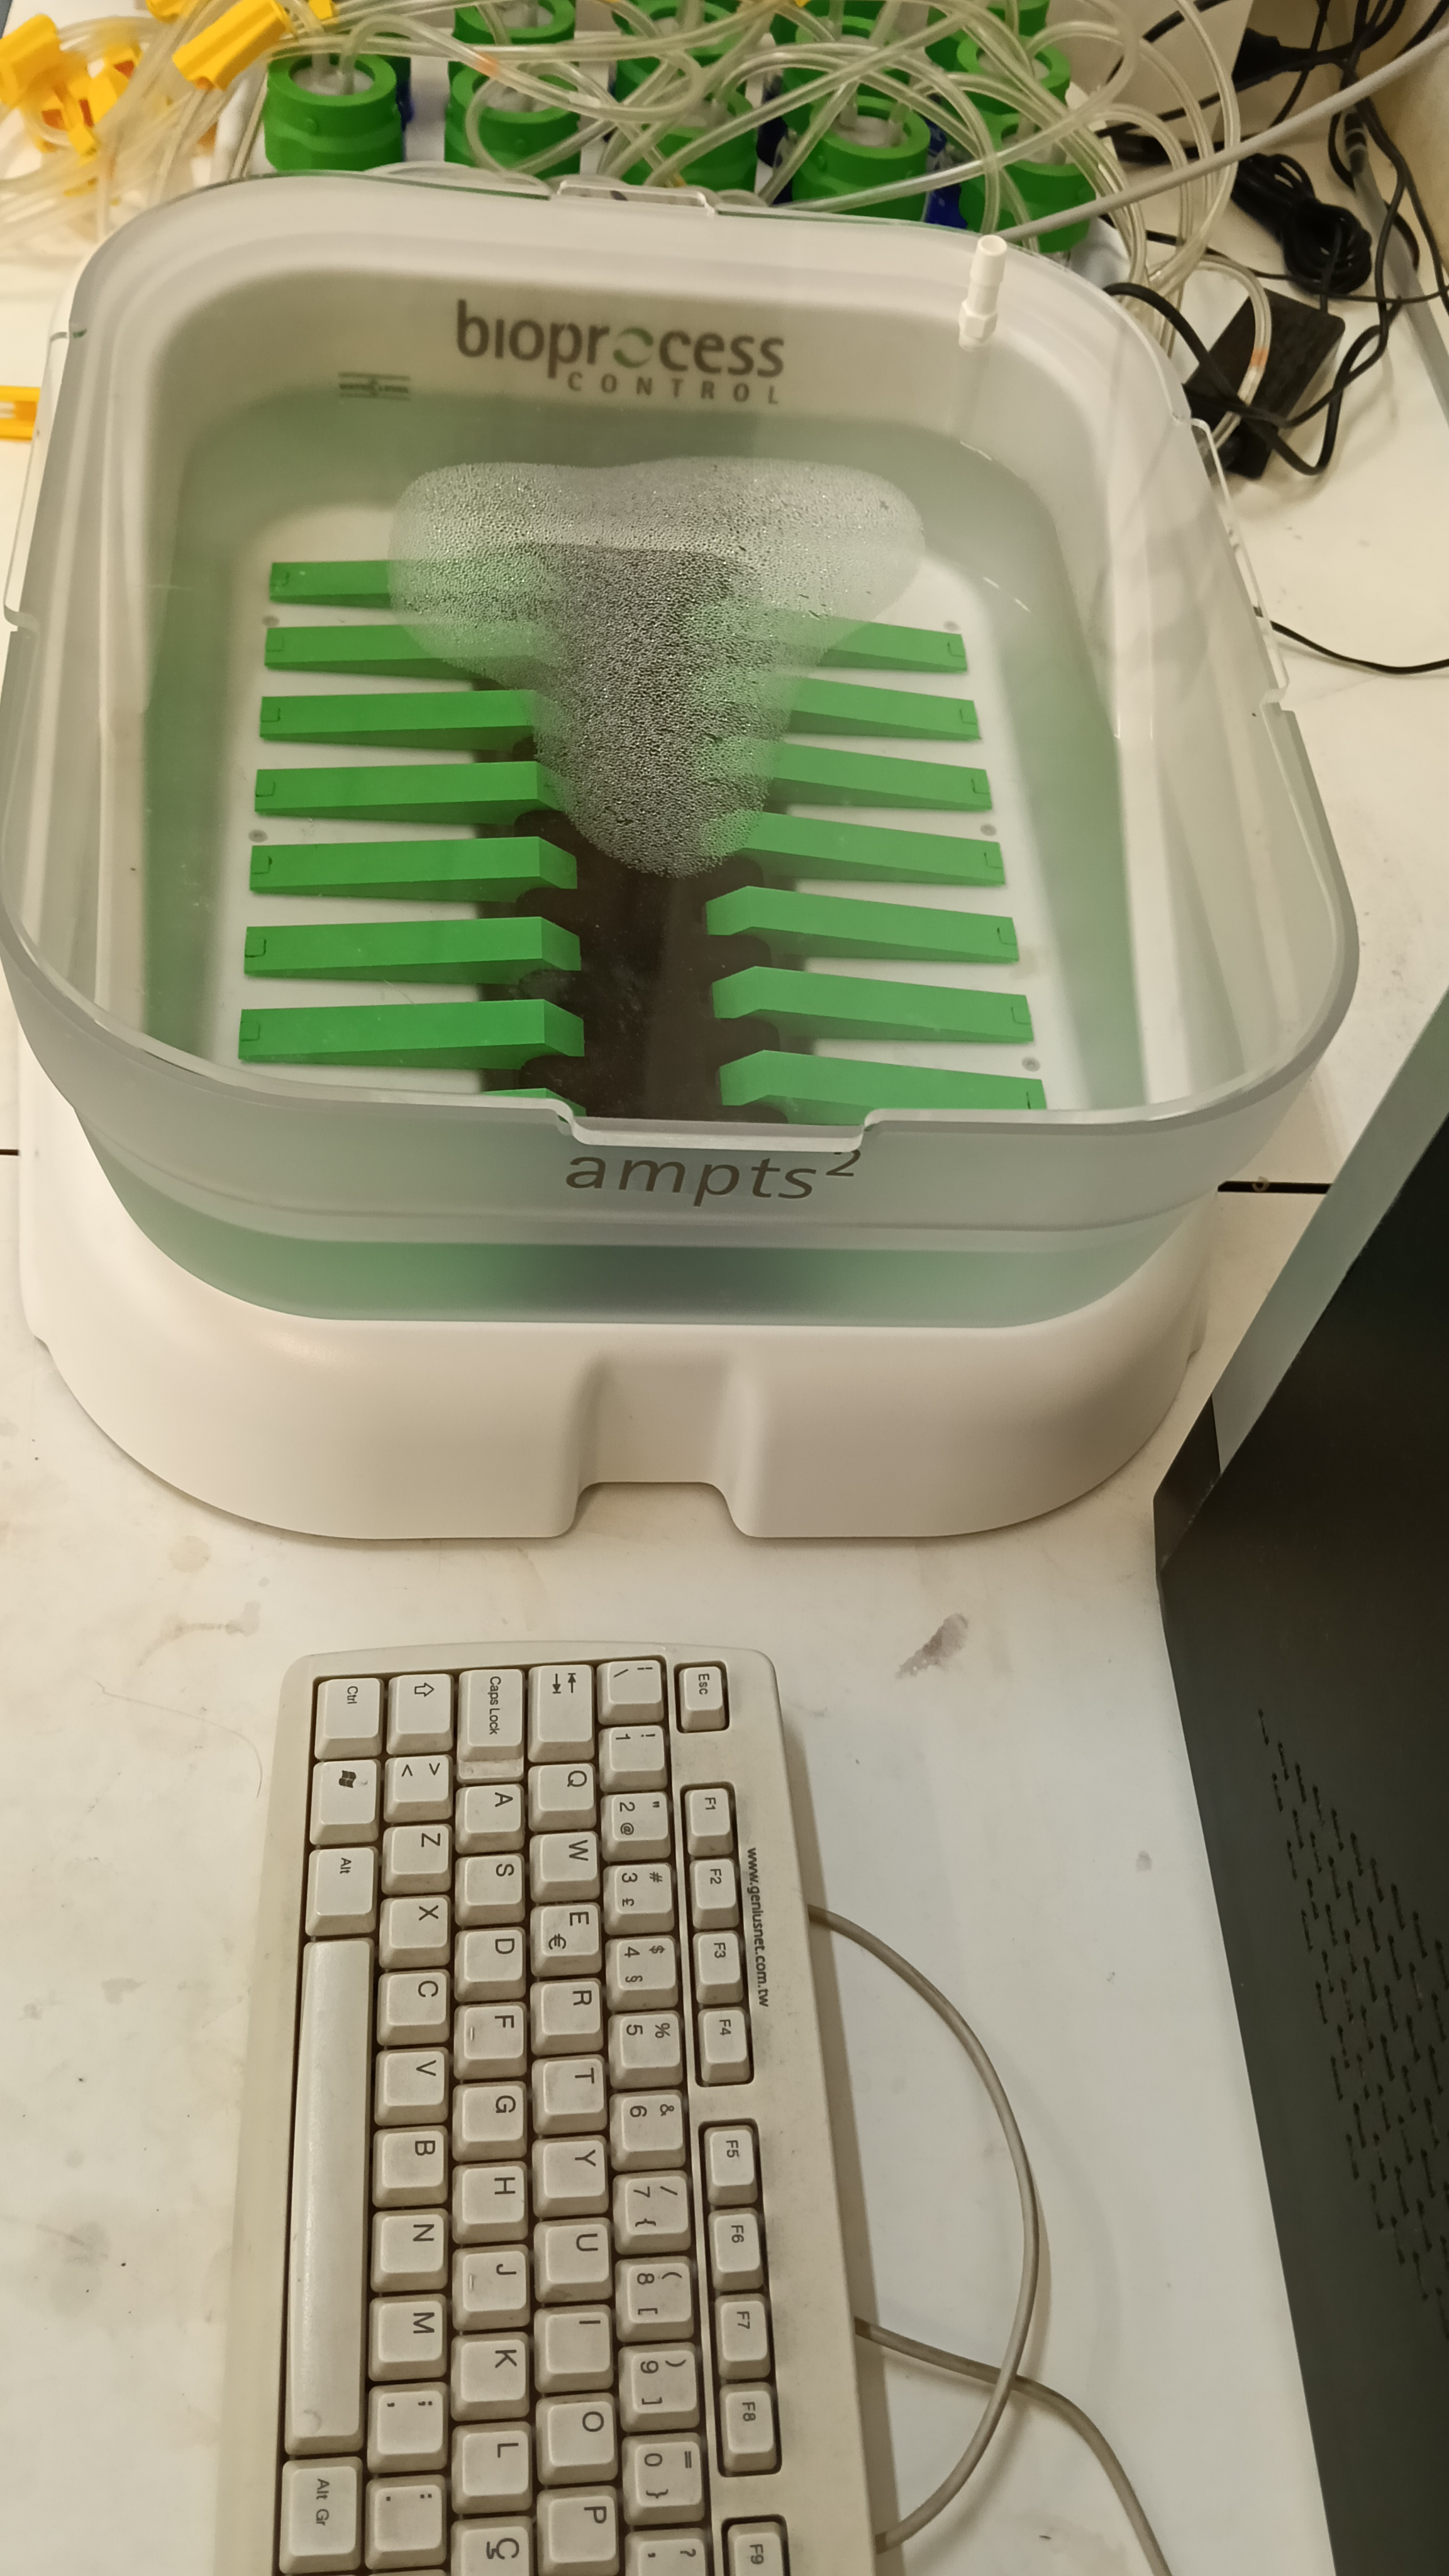
\includegraphics[width=0.6\textwidth]{assets/ampts.jpg}
    \caption{Source: Author}
    \label{fig:ampts}
\end{figure}

\subsection{Analysis Methods}
\label{subsec:analysis_methods}

It was used the method of DiLallo \& Albertson \parencite{ribas2007}, to measure the alkalinity and volatile fatty acids. The sample collected was first centrifuged, at \qty{2604}{\gforce} for \qty{30}{\minute}, to filter the particulated before doing the measurements.

\begin{equation}
    \text{TA} = \frac{N_\text{acid} * V_\text{acid} * 50000}{V_\text{sample}}
    \label{eq:TA}
\end{equation}
\begin{equation}
    \text{VFA} = \frac{N_\text{base} * V_\text{base} * 60000}{V_\text{sample}}
    \label{eq:VFA}
\end{equation}

The volumes were measured in \unit{\milli\litre}, the sample volume was always \qty{50}{\milli\litre}, the normality (\unit{\normality}) of the acid and base, at first was \num{0.1}, but then it was changed to \num{1}. The \cref{eq:TA} is expressed in \unit{\milli\gram\ce{CaCO3}\per\litre}, and the \cref{eq:VFA} is expressed in \unit{\milli\gram\ce{CH3COOH}\per\litre}.

\subsection{Subestrate used as feed}
\label{subsec:sub_feed}

\Cref{tab:feeds} shows all substrates used to feed the reactor and when they were made.

\begin{footnotesize} % TODO transformar em uma tabela csv para facilitar o trabalho
    \begin{ThreePartTable}
        \begin{xltabular}{\linewidth}{@{} C C C C C C C @{}}

        \caption{Substrates used during the process}
        \label{tab:feeds} \\

        \toprule
        \thead{Day} &
        \thead{Substrate 1} &
        \thead{Subestrate 2} &
        \thead{Substrate 3} &
        \thead{Extra\\ Addition} &
        \thead{COV\\ \& TS\%} &
        \thead{Volume\\ Made} \\
        \midrule
        \endfirsthead

        \multicolumn{6}{l}{\textit{\Cref{tab:feeds} continued}} \\
        \toprule
        \thead{Day} &
        \thead{Substrate 1} &
        \thead{Subestrate 2} &
        \thead{Substrate 3} &
        \thead{Extra\\ Addition} &
        \thead{COV\\ \& TS\%} &
        \thead{Volume\\ Made} \\
        \midrule
        \endhead

        \bottomrule
        \endlastfoot

        0\tnote{a} &
        Food Waste, 156 g &
        Glucose, 1.9 g &
        &
        Calcium Bicarbonate, 5 g &
        1.5 \& 15 &
        500 mL\\
        \addlinespace
        4 &
        Crude Glicerol, \approx 23.2 mL &
        Pure Glicerol\tnote{b}, \approx 31.5 mL &
        &
        Potassium Bicarbonate, \approx 1.9 g &
        0.8 \& 10 &
        250 mL\\
        \addlinespace
        11 &
        Food Waste, \approx 12.54 g &
        Crude Glicerol, \approx 9.02 mL &
        Pure Glicerol, \approx 2.6 mL &
        Potassium Bicarbonate, \approx 1.57 g &
        0.13-0.4 \& 5-10 &
        250 mL\\
        \addlinespace
        18 &
        Food Waste, \approx 10.88 g &
        Crude Glicerol, \approx 2.89 mL &
        Pure Glicerol, \approx 1.44 mL &
        &
        0.0256 \& \approx 2 &
        250 mL\\
        \addlinespace
        25 &
        Food Waste, \approx 31.12 g &
        Crude Glicerol, \approx 44 mL &
        Pure Glicerol, \approx 29 mL &
        &
        \approx 1.4 \& \approx 10 &
        250 mL \\
        \addlinespace
        32 &
        Food Waste, \approx 31.01 g &
        Crude Glicerol, \approx 44 mL &
        Pure Glicerol, \approx 28.9 mL &
        &
        \approx 1.4 \& \approx 10 &
        250 mL \\
        \addlinespace
        39 &
        Food Waste, \approx 46.52 g &
        Crude Glicerol, \approx 66 mL &
        Pure Glicerol, \approx 43 mL &
        Potassium Bicarbonate, \approx 2.6 g &
        \approx 3.1 \& \approx 15 &
        250 mL \\
        \addlinespace
        46 &
        Food Waste, \approx 50.07 g &
        Crude Glicerol, \approx 66 mL &
        Pure Glicerol, 43 mL &
        Potassium Bicarbonate, \approx 2.67 g &
        \approx 3.16 \& \approx 15 &
        250 mL \\
        \addlinespace
        53\tnote{c} &
        Crude Glicerol, \approx 55 mL &
        Pure Glicerol, \approx 11.5 mL &
        &
        Potassium Bicarbonate, \approx 5.38 g &
        0.42 \& \approx 10 &
        500 mL \\
        \addlinespace
        60 &
        Crude Glicerol, \approx 55 mL &
        Pure Glicerol, \approx 12 mL &
        &
        Potassium Bicarbonate, \approx 5.18 g &
        0.42 \& \approx 10 &
        500 mL\tnote{d} \\
        \addlinespace
        67 &
        Crude Glicerol, \approx 41 mL &
        Pure Glicerol, \approx 9 mL &
        &
        Potassium Bicarbonate, \approx 2.56 g &
        0.95 \& \approx 15 &
        250 mL \\
        \addlinespace
        74 &
        Crude Glicerol, \approx 60 mL &
        Pure Glicerol, \approx 12.5 mL &
        &
        Potassium Bicarbonate, \approx 2.57 g &
        \approx 1.37 \& \approx 15 &
        250 mL \\

        \end{xltabular}

        \begin{tablenotes}
            \item[a] It only started feeding on day 2.
            \item[b] The solution of pure glicerol was diluted 100X.
            \item[c] Change of substrate.
            \item[d] There was a leak on the feeding tube.
            \newline
            \item Source: Author
        \end{tablenotes}
    \end{ThreePartTable}
\end{footnotesize}
